\section*{15/11}
	
	\[
	\int B^TDB\ dV
	\]
	\[
	B=\begin{bmatrix}
		\dfrac{\partial\left[ N \right]}{\partial x} \\  \\ \dfrac{\partial\left[ N \right]}{\partial y}
	\end{bmatrix} \qquad \text{ где } \hspace{3mm} \begin{matrix}
	N_1 = L_1(2L_1-1) \\ N_3 = L_2(2L_2-1) \\ N_5=L_3(2L_3-1)
	\end{matrix} \quad \begin{matrix}
	N_2 = 4L_1L_2 \\ N_4 = 4L_2L_3 \\ N_6=4L_3L_1
	\end{matrix}
	\]
	\[
	\begin{cases}
		x=x(L_1,L_2,L_3) \\
		y=y(L_1,L_2,L_3) 
	\end{cases}
	\]
	
	$\beta=\overline{1, 6}:$
	\[
	\begin{cases}
		\frac{\partial N_{\beta}}{\partial L_1} = \frac{\partial N_{\beta}}{\partial x} \cdot \frac{\partial x}{\partial L_1} + \frac{\partial N_{\beta}}{\partial y} \cdot \frac{\partial y}{\partial L_1} \\
		\frac{\partial N_{\beta}}{\partial L_2} = \frac{\partial N_{\beta}}{\partial x} \cdot \frac{\partial x}{\partial L_2} + \frac{\partial N_{\beta}}{\partial y} \cdot \frac{\partial y}{\partial L_2}
	\end{cases} \quad \Leftrightarrow \quad \begin{bmatrix}
	\frac{\partial N_{\beta}}{\partial L_1} \\ \frac{\partial N_{\beta}}{\partial L_2}
	\end{bmatrix} = \underbrace{\begin{bmatrix}
	\frac{\partial x}{\partial L_1} & \frac{\partial y}{\partial L_1} \\ \frac{\partial x}{\partial L_2} & \frac{\partial y}{\partial L_2} 
	\end{bmatrix}}_J \cdot \begin{bmatrix}
 	\frac{\partial N_{\beta}}{\partial x} \\ \frac{\partial N_{\beta}}{\partial y}
	\end{bmatrix}
	\]
	\[
	\begin{bmatrix}
		\frac{\partial N_{\beta}}{\partial x} \\ \frac{\partial N_{\beta}}{\partial y}
	\end{bmatrix} = J^{-1} \cdot \begin{bmatrix}
	\frac{\partial N_{\beta}}{\partial L_1} \\ \frac{\partial N_{\beta}}{\partial L_2}
	\end{bmatrix}
	\]
	\[
	\frac{\partial N_{\beta}}{\partial L_1}= \frac{\partial N_{\beta}}{\partial L_1}\cdot \underbrace{\frac{\partial L_1}{\partial L_1}}_1 + \frac{\partial N_{\beta}}{\partial L_2}\cdot \underbrace{\frac{\partial L_2}{\partial L_1}}_0+\frac{\partial N_{\beta}}{\partial L_3}\cdot \underbrace{\frac{\partial L_3}{\partial L_1}}_{-1}=\frac{\partial N_{\beta}}{\partial L_1}-\frac{\partial N_{\beta}}{\partial L_3}
	\]
	\underline{Пример:}
	\[
	N_4=4L_2L_3=4L_2(1-L_1-L_2)\Rightarrow \frac{\partial N_4}{\partial L_1}=-4L_2
	\]
	\[
	Z=\int\limits_0^1\int\limits_0^{1-L_2} f(L_1, L_2, L_3)|J|\ dL_1dL_2 = \sum\limits_{i=1}^{n} W_i g (L_1,L_2,L_3), \text{ где } g=f\cdot|J|
	\]
	\begin{center}
	\begin{tabular}{|c|c|c|c|c|}
		\hline
		& Ошибка & ($\cdot$) & $L_1\ L_2\ L_3$ & $W_i$ \\
		\hline
		\raisebox{-10mm}{%
		\begin{tikzpicture}
			% Координаты вершин треугольника
			\coordinate (A) at (0,0);
			\coordinate (B) at (2,0);
			\coordinate (C) at (1,1.5);
			
			% Центр треугольника (среднее арифметическое координат вершин)
			 \coordinate (O) at ($ (A)!0.333!(B) + (A)!0.333!(C) + (B)!0.333!(C) $);
			
			% Рисуем треугольник
			\draw[thick] (A) -- (B) -- (C) -- cycle;
			
			% Координаты середин сторон
			\coordinate (a) at ($(B)!0.5!(C)$);
			\coordinate (b) at ($(A)!0.5!(C)$);
			\coordinate (c) at ($(A)!0.5!(B)$);
			
			% Векторы от середины сторон к центру
			\draw[->, thick] (a) -- (1, 0.5);
			\draw[->, thick] (b) -- (1, 0.5);
			\draw[->, thick] (c) -- (1, 0.5);
			
			% Обозначения середин сторон
			\node[anchor=west] at (a) {$L_1$};
			\node[anchor=east] at (b) {$L_2$};
			\node[anchor=north] at (c) {$L_3$};
			

		\end{tikzpicture}} & $R=o(h^2)$ & a & $\frac{1}{3}\ \frac{1}{3}\ \frac{1}{3}$ & $\frac{1}{2}$ \\
		\hline
		\raisebox{-10mm}{%
		\begin{tikzpicture}
			% Координаты вершин треугольника
			\coordinate (A) at (0,-1);
			\coordinate (B) at (2,-1);
			\coordinate (C) at (1,0.5);
			
			% Рисуем треугольник
			\draw[thick] (A) -- (B) -- (C) -- cycle;
			
			% Координаты середин сторон
			\coordinate (a) at ($(B)!0.5!(C)$);
			\coordinate (b) at ($(A)!0.5!(C)$);
			\coordinate (c) at ($(A)!0.5!(B)$);
			
			% Обозначения точек в серединах сторон
			\node[anchor=west] at (a) {$c$};
			\node[anchor=east] at (b) {$a$};
			\node[anchor=north] at (c) {$b$};
			
			% Точки на серединах
			\fill (a) circle (2pt);
			\fill (b) circle (2pt);
			\fill (c) circle (2pt);
		\end{tikzpicture}
	}
		& \makecell{\textcolor{white}{a}\\  $R=o(h^2)$ \\ \textcolor{white}{a} }  
		& \makecell{a \\ b \\ c} 
		& \makecell{$\frac{1}{2}\ 0\ \frac{1}{2}$ \\ $\frac{1}{2}\ \frac{1}{2}\ 0$ \\ $0\ \frac{1}{2}\ \frac{1}{2}$} 
		& \makecell{$\frac{1}{6}$ \\ $\frac{1}{6}$ \\ $\frac{1}{6}$} \\
		
		 \hline
		  \raisebox{-5mm}{%
		 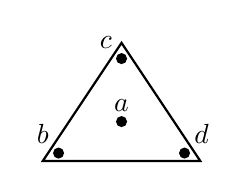
\begin{tikzpicture}
		 	% Координаты вершин треугольника
		 	\coordinate (A) at (0,0);
		 	\coordinate (B) at (2,0);
		 	\coordinate (C) at (1,1.5);
		 	
		 	% Рисуем треугольник
		 	\draw[thick] (A) -- (B) -- (C) -- cycle;
		 	
		 	% Координаты середин сторон
		 	\coordinate (a) at (1, 0.5);
		 	\coordinate (b) at (0.2, 0.1);
		 	\coordinate (c) at (1, 1.3);
		 	\coordinate (d) at (1.8, 0.1);
		 	
		 	% Обозначения точек в серединах сторон
		 	\node[anchor=south] at (a) {$a$};
		 	\node[anchor=south east] at (b) {$b$};
		 	\node[anchor=south east] at (c) {$c$};
		 	\node[anchor=south west] at (d) {$d$};
		 	
		 	% Точки на серединах
		 	\fill (a) circle (2pt);
		 	\fill (b) circle (2pt);
		 	\fill (c) circle (2pt);
		 	\fill (d) circle (2pt);
		 \end{tikzpicture}} & \makecell{\textcolor{white}{a}\\  $R=o(h^4)$ \\ \textcolor{white}{a} } & \makecell{a \\ b \\ c \\ d}  & \makecell{$\frac{1}{3}\ \frac{1}{3}\ \frac{1}{3}$ \\ $\frac{11}{15}\ \frac{2}{15}\ \frac{2}{15}$ \\ $\frac{2}{15}\ \frac{2}{15}\ \frac{11}{15} $ \\ $\frac{2}{15}\ \frac{11}{15}\ \frac{2}{15} $} & \makecell{  $\frac{27}{96}$\\ $\frac{25}{96}$ \\ $\frac{25}{96}$ \\ $\frac{25}{96}$  } \\
		 
		 \hline
		 \raisebox{-10mm}{%
		 \begin{tikzpicture}
		 	% Координаты вершин треугольника
		 	\coordinate (A) at (0,0);
		 	\coordinate (B) at (2,0);
		 	\coordinate (C) at (1,1.5);
		 	
		 	% Рисуем треугольник
		 	\draw[thick] (A) -- (B) -- (C) -- cycle;
		 	
		 	% Координаты середин сторон
		 	\coordinate (a) at (1, 0.5);
		 	\coordinate (b) at ($(A)!0.5!(C)$);
		 	\coordinate (c) at ($(B)!0.5!(C)$);
		 	\coordinate (d) at ($(A)!0.5!(B)$);
		 	\coordinate (e) at (1, 1.5);
		 	\coordinate (f) at (0, 0);
		 	\coordinate (g) at (2, 0);
		 
		 	% Обозначения точек в серединах сторон
		 	\node[anchor=south] at (a) {$a$};
		 	\node[anchor=south east] at (b) {$b$};
		 	\node[anchor=south west] at (c) {$c$};
		 	\node[anchor=north] at (d) {$d$};
		 	\node[anchor=south] at (e) {$e$};
		 	\node[anchor=north] at (f) {$f$};
		 	\node[anchor=north] at (g) {$g$};
		 	
		 	% Точки на серединах
		 	\fill (a) circle (2pt);
		 	\fill (b) circle (2pt);
		 	\fill (c) circle (2pt);
		 	\fill (d) circle (2pt);
		 	\fill (e) circle (2pt);
		 	\fill (f) circle (2pt);
		 	\fill (g) circle (2pt);
		 \end{tikzpicture}} & \makecell{\textcolor{white}{a}\\  $R=o(h^4)$ \\ \textcolor{white}{a} }   & \makecell{a \\ b \\ c \\ d \\ e \\ f \\ g} & \makecell{ $\frac{1}{3}\ \frac{1}{3}\ \frac{1}{3}$ \\ $\frac{1}{2}\ 0\ \frac{1}{2}$ \\ $0\ \frac{1}{2}\ \frac{1}{2} $ \\ $\frac{1}{2}\ \frac{1}{2}\ 0 $ \\ $0\ 0\ 1 $ \\ $1\ 0\ 0 $ \\ $0\ 1\ 0 $}  & \makecell{$\frac{27}{120}$ \\ $\frac{8}{120}$ \\ $\frac{8}{120}$ \\  $\frac{8}{120}$ \\ $\frac{3}{120}$ \\  $\frac{3}{120}$ \\ $\frac{3}{120}$ } \\
		 
		 \hline
		 \raisebox{-10mm}{%
		 	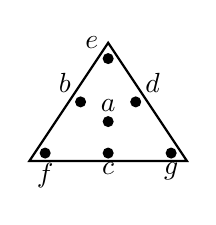
\begin{tikzpicture}
		 		% Координаты вершин треугольника
		 		\coordinate (A) at (0,0);
		 		\coordinate (B) at (2,0);
		 		\coordinate (C) at (1,1.5);
		 		
		 		% Рисуем треугольник
		 		\draw[thick] (A) -- (B) -- (C) -- cycle;
		 		
		 		% Координаты середин сторон
		 		\coordinate (a) at (1, 0.5);
		 		\coordinate (b) at (0.65, 0.75);
		 		\coordinate (c) at (1, 0.1);
		 		\coordinate (d) at (1.35, 0.75);
		 		\coordinate (e) at (1, 1.3);
		 		\coordinate (f) at (0.2, 0.1);
		 		\coordinate (g) at (1.8, 0.1);
		 		
		 		% Обозначения точек в серединах сторон
		 		\node[anchor=south] at (a) {$a$};
		 		\node[anchor=south east] at (b) {$b$};
		 		\node[anchor=north] at (c) {$c$};
		 		\node[anchor=south west] at (d) {$d$};
		 		\node[anchor=south east] at (e) {$e$};
		 		\node[anchor=north] at (f) {$f$};
		 		\node[anchor=north] at (g) {$g$};
		 		
		 		% Точки на серединах
		 		\fill (a) circle (2pt);
		 		\fill (b) circle (2pt);
		 		\fill (c) circle (2pt);
		 		\fill (d) circle (2pt);
		 		\fill (e) circle (2pt);
		 		\fill (f) circle (2pt);
		 		\fill (g) circle (2pt);
		 \end{tikzpicture} } & \makecell{\textcolor{white}{a}\\  $R=o(h^6)$ \\   $\alpha=0.05961587$ \\ $\beta=0.47014206$ \\ $\gamma=0.10128651$ \\ $\Delta=0.79742699$\\ \textcolor{white}{a}}   & \makecell{a \\ b \\ c \\ d \\ e \\ f \\ g} & \makecell{ $\frac{1}{3}\ \frac{1}{3}\ \frac{1}{3}$ \\ $\beta\ \alpha\ \beta$ \\ $\beta\ \beta\ \alpha$ \\ $\alpha\ \beta\ \beta$ \\ $\gamma\ \gamma\ \delta$ \\ $\delta\ \gamma\ \gamma\ $ \\ $\gamma\ \delta\ \gamma\ $} & \makecell{ $0.1125$ \\  $0.066197075$ \\ $0.066197075$ \\ $0.066197075$ \\ $0.0629695$ \\ $0.0629695$ \\ $0.0629695$  } \\
		  \hline 
	\end{tabular}
	\end{center}
	
	\newpage
	\underline{Пример.} 
	\[
	\text{Вычислить: }\int\limits_S \frac{\partial N_4}{\partial x}\cdot\frac{\partial N_4}{\partial y}\ dxdy
	\]
	\begin{figure}[H]
	\begin{minipage}{0.45\textwidth}
	\begin{center}
	
	\begin{tikzpicture}
		% Координаты вершин треугольника
		\coordinate (A) at (0,0); % Вершина A
		\coordinate (B) at (2,0); % Вершина B
		\coordinate (C) at (1,1.5); % Вершина C
		
		
		% Рисуем оси
		\draw[->] (-1,-1) -- (3,-1) node[anchor=west] {$x$}; % Ось x
		\draw[->] (-1,-1) -- (-1,2) node[anchor=south] {$y$}; % Ось y
		
		% Рисуем треугольник
		\draw[thick] (A) -- (B) -- (C) -- cycle;
		
		% Координаты середин сторон
		\coordinate (a) at ($(B)!0.5!(C)$); % середина BC
		\coordinate (b) at ($(A)!0.5!(C)$); % середина AC
		\coordinate (c) at ($(A)!0.5!(B)$); % середина AB
		
		% Обозначения вершин
		\node[anchor=north east] at (A) {$1$};
		\node[anchor=north west] at (B) {$3$};
		\node[anchor=south] at (C) {$5$};
		
		% Обозначения середин сторон
		\node[anchor=west] at (a) {$4$};
		\node[anchor=east] at (b) {$6$};
		\node[anchor=north] at (c) {$2$};
		
		\fill (a) circle (2pt);
		\fill (b) circle (2pt);
		\fill (c) circle (2pt);
		\fill (A) circle (2pt);
		\fill (B) circle (2pt);
		\fill (C) circle (2pt);
		
	\end{tikzpicture} 
	\end{center}
	\end{minipage}
	\begin{minipage}{0.45\textwidth}
	\begin{center}
	\begin{tabular}{c|c}

		Точка & Координаты точки \\
		\hline
		1 & 1 \qquad 1 \\
		\hline
		3 & 3 \qquad 2 \\
		\hline
		5 & 2 \qquad 3 \\
	\end{tabular}
	\end{center}
	\end{minipage}
	\end{figure}
	\[
	\begin{cases}
		x=x_1L_1+x_3L_2+x_5L_3 \\
		y = y_1L_1+y_3L_2+y_5L_3 
	\end{cases}
	\Rightarrow \begin{cases}
		x=L_1+3L_2+2L_3 \\
		y=L_1+2L_3+3L_3
	\end{cases}
	\]
	\[
	N_4=4L_2L_3
	\]
	\[
	J=\begin{bmatrix}
		\frac{\partial x}{\partial L_1} & \frac{\partial y}{\partial L_1} \\
		\frac{\partial x}{\partial L_2} & \frac{\partial y}{\partial L_2}
	\end{bmatrix} = \begin{bmatrix}
	1-2 & 1-3 \\ 3-2 & 2-3 
	\end{bmatrix} = \begin{bmatrix}
	-1 & -2 \\ 1 & -1
	\end{bmatrix} \Rightarrow |J|=1+2=3
	\]
	\[
	\begin{bmatrix}
		\frac{\partial N_4}{\partial x} \\ \frac{\partial N_4}{\partial y}
	\end{bmatrix} = \frac{1}{3} \begin{bmatrix}
	-1 & -1 \\ 2 & -1 
	\end{bmatrix}\begin{bmatrix}
	-4L_2 \\ 4L_3-4L_2
	\end{bmatrix} \Rightarrow 
	\] 
	\[
	\frac{\partial N_4}{\partial x}=\frac{1}{3}(8L_2-4L_3) \qquad 
	\frac{\partial N_4}{\partial  y}=\frac{-1}{3}(4L_2+4L_3)
	\]
	\[
	\frac{\partial N_4}{\partial x}\cdot\frac{\partial N_4}{\partial y}=-\frac{1}{9}(8L_2-4L_3)(4L_2+4L_3)=\int\limits_S \frac{\partial N_4}{\partial x}\cdot\frac{\partial N_4}{\partial y}\ dxdy = 
	\]
	\[
	=\int\limits_0^1\int\limits_0^{1-L_2} -\frac{1}{9}\cdot 3 (8L_2-4L_3)(4L_2+4L_3) \ dL_1dL_2 = -\frac{1}{3} \sum\limits_{i=1}^{3} W_i\cdot g(L_1, L_2, L_3) = -\frac{12}{18}
	\]